\documentclass[11pt, twoside]{book}
\usepackage[full]{leadsheets}
\usepackage[a4paper,  hmargin=1.5cm, vmargin=3cm, head=14pt, foot=50pt]{geometry}
\usepackage{multicol}
\usepackage[polish]{babel}
\usepackage{array}
\usepackage{graphicx}
\usepackage{hyperref}
\usepackage{tocloft}
%\usepackage[toc]{multitoc}
\usepackage{fancyhdr}
\usepackage{tikzpagenodes}
\usepackage{titlesec}
\usepackage{tabularx}
\usepackage{adjustbox}
\usepackage{tipa}
\usepackage{ifxetex}
\usepackage{changepage}
\usepackage[version=4]{mhchem}
\usepackage[%
    left = „,%
    right = “,%
    leftsub = «,%
    rightsub = »%
]{dirtytalk}

\thispagestyle{empty}

\ifxetex%
    \usepackage{substitutefont}
    \substitutefont{T3}{\rmdefault}{cmr}
\fi

%\usepackage[T1]{fontenc}

\selectlanguage{polish}
\DeclareTranslation{Polish}{leadsheets/chorus}{Ref.}
\DeclareTranslation{Polish}{leadsheets/interlude}{Przej.}
\DeclareTranslation{Polish}{leadsheets/bridge}{Bridge}
\DeclareTranslation{Polish}{leadsheets/lyrics}{tekst}
\DeclareTranslation{Polish}{leadsheets/verse}{Zwr.}
\DeclareTranslation{Polish}{leadsheets/capo}{Capo}
\DeclareTranslation{Polish}{leadsheets/fret}{próg}

% Tytuł spisu treści
\addto\captionspolish{\renewcommand*\contentsname{Jakieś piosenki}}

% Flaga oznaczająca, czy dany utwór ma mieć symbol odnoszący do aneksu
\definesongproperty{annex}

\definesongtitletemplate{custom}{%
    \let\clearpage\relax
    \ifsongmeasuring%
        {\section*}
        {\section}%
        {\songproperty{title}}%
    \begingroup\footnotesize
        \begin{tabular}{%
                @{}
                >{\raggedright\arraybackslash}p{.5\linewidth}
                @{}
                >{\raggedleft\arraybackslash}p{.5\linewidth}
                @{}
            }
            \ifsongproperty{music}{%
                Muzyka: \songproperty{music}
                }{}%
            \ifsongproperty{annex}{%
                &
                \smash{\includegraphics[height=40pt]{images/aneks-ref.png}}
                }{}%
            \ifsongproperty{music}{\\}{\ifsongproperty{annex}{\\}{}}%
            \ifsongproperty{lyrics}{%
                Tekst: \songproperty{lyrics} \\%
                }{}%
            \ifsongproperty{interpret}{%
                Interpretacja: \songproperty{interpret} \\%
                }{}%
            \ifsongproperty{capo}{%
                \capo{} \\%
                }{}%
        \end{tabular}%
        \par
    \endgroup
}

\setleadsheets{%
    title-template = custom,
    verse/numbered,
    remember-chords = false,
    align-chords = {l},
    capo-nr-format = arabic,
    bar-shortcuts
}
\setchords{%
    minor = {lowercase},
    input-notation = german,
    output-notation = german
}

\renewcommand{\chaptermark}[1]{\markboth{#1}{}}

\fancypagestyle{plain}{%
    \fancyhf{}
    \fancyhead[L]{Jakieś piosenki}
    \fancyfoot[LE,RO]{\Large\thepage}
}
\fancypagestyle{szanty}{%
    \pagestyle{plain}
    \fancyhead[R]{Szanty}
    \fancyfoot[LO]{\includegraphics[height=45pt]{images/kolo.png}}
    \fancyfoot[RE]{\includegraphics[height=45pt]{images/kotwica.png}}
}
\fancypagestyle{poezja}{%
    \pagestyle{plain}
    \fancyhead[R]{Poezja śpiewana}
    \fancyfoot[LO]{\includegraphics[height=45pt]{images/wilk.png}}
    \fancyfoot[RE]{\includegraphics[height=45pt]{images/drzewa.png}}
}
\fancypagestyle{pop}{%
    \pagestyle{plain}
    \fancyhead[R]{Pop}
    \fancyfoot[LO]{\includegraphics[height=45pt]{images/gwiazdy.png}}
    \fancyfoot[RE]{\includegraphics[height=45pt]{images/gitara.png}}
}
\fancypagestyle{autorskie}{%
    \pagestyle{plain}
    \fancyhead[R]{Autorskie}
    \fancyfoot[LO]{
\includegraphics[height=45pt]{images/kalamarz.jpeg}}
    \fancyfoot[RE]{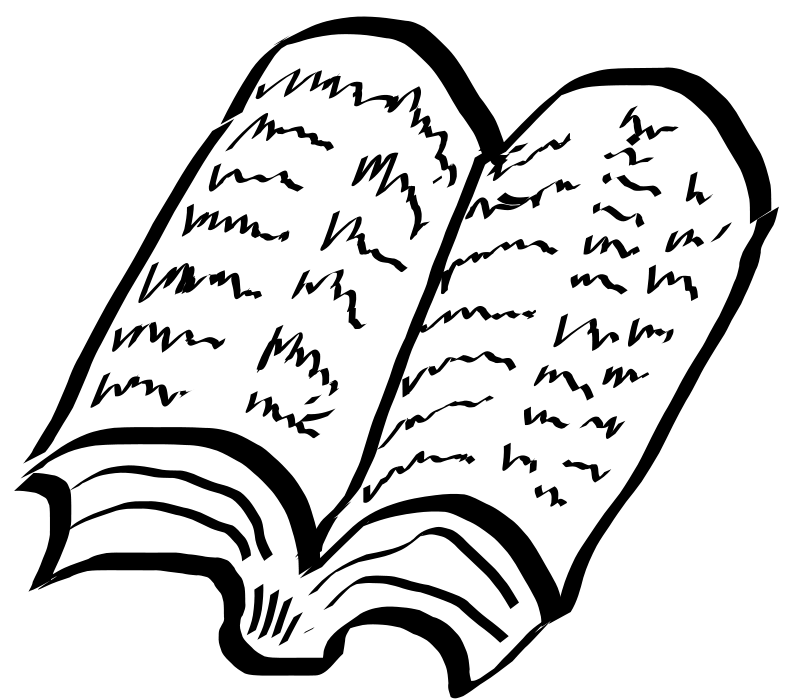
\includegraphics[height=45pt]{images/ksiazka_bazgroly.png}}
}
\fancypagestyle{legendy}{%
    \pagestyle{plain}
    \fancyhead[R]{Legendy, opowieści, ciekawostki}
    \fancyfoot[LO]{\includegraphics[height=45pt]{images/swieczka.png}}
    \fancyfoot[RE]{\includegraphics[height=45pt]{images/fajka.png}}
}

\renewcommand{\cftdot}{\ensuremath{\sim}}
\renewcommand{\cftsecleader}{\cftdotfill{\cftdotsep}}

% Usunięcie numeru rozdziału sprzed numeru sekcji
%\renewcommand{\thesection}{\arabic{section}}

\titleformat{\chapter}[block]{\centering\vspace{6cm}}{}{0pt}{\Huge\bfseries}

\newversetype{riff}[name={Riff}, numbered=false, named=true]

\counterwithin*{footnote}{section}

% Pionowy apostrof do angielskiego i francuskiego
\newcommand{\tqs}{\textquotesingle}

\begin{document}

\begin{titlepage}
    \begin{center}
        \vspace*{5cm}
        
        \includegraphics[height=8cm]{images/front-obrazek.png}

        \vspace{1.5cm}

        \Huge\textbf{Jakieś piosenki}
        
        \vspace{0.5cm}
        
        \large Wydanie pierwsze \\
        \small Podwydanie pierwsze
        
        \vfill

        \large
        Wydawnictwo Kis Inkris \\
        Warszawa, 2023

        \vspace{0.8cm}

        \footnotesize
        \textit{%
        Gdzie słyszysz śpiew, tam wejdź, tam dobre serce mają \\
        Żli ludzie, wierzaj mi, ci nigdy nie śpiewają} \medskip \\
        Johann Gottfried Seume, \textit{Die Gesänge}

    \end{center}
\end{titlepage}

\pagestyle{plain}

\tableofcontents
\vfill
\renewcommand{\tabularxcolumn}[1]{>{\small}b{#1}}
\begin{adjustbox}{width={\textwidth}, keepaspectratio}
\begin{tabularx}{\textwidth}{%
        @{}
        >{\raggedright\arraybackslash}X
        @{}
        >{\raggedleft\arraybackslash}X
    }
    \footnotesize
    Kamil Dzierżanowski \hfill opracowanie, skład, korekta

    Paweł Kulig \hfill opracowanie

    Piotr Wieżel \hfill opracowanie
    
    Mateusz Dorobek \hfill opracowanie

    \medskip

    Daj śpiewnikowi gwiazdkę na GitHubie:

    \smallskip

    \urlstyle{same}
    \url{https://github.com/dzierzanowski/spiewnik-szant}

    \bigskip

    Dziękujemy za grafiki z Freepik od dgim-studio i pch.vector!

    &

    Pobierz śpiewnik online:

    \smallskip

    \includegraphics[width=3cm]{images/qr.png}
\end{tabularx}
\end{adjustbox}

\chapter{Szanty}
\begin{center}
    \includegraphics[width=0.5\textwidth]{images/wezel.png}
\end{center}
\pagestyle{szanty}
\input{songs/trzy_majtki-24_lutego}
\input{songs/mechanicy_shanty-bitwa}
\input{songs/mietek_folk-chlopcy_z_botany_bay}
\input{songs/trzy_majtki-cztery_piwka}
\input{songs/krzysztof_klenczon-dziesiec_w_skali_beauforta}
\input{songs/ryczace_dwudziestki-few_days}
\input{songs/trzy_majtki-gdzie_ta_keja}
\input{songs/ryczace_dwudziestki-hiszpanskie_dziewczyny}\newpage\pagestyle{szanty}
\input{songs/ryczace_dwudziestki-jasnowlosa}
\input{songs/ekt_gdynia-ja_stawiam}
\input{songs/north_cape-kapitan_kidd}
\input{songs/perly_i_lotry-la_valette}
\input{songs/ekt_gdynia-male_piwo}
\input{songs/mechanicy_shanty-marco_polo}
\input{songs/ekt_gdynia-morze_moje_morze}
\input{songs/artur_andrus-nazywali_go_marynarz}
\input{songs/mechanicy_shanty-pacyfik}
\input{songs/ekt_gdynia-piesn_wielorybnikow}\newpage\pagestyle{szanty}
\input{songs/poszedlem_na_dziob-pij_za_starego}
\input{songs/cztery_refy-pozegnanie_liverpoolu}
\input{songs/cztery_refy-press_gang(branka)}
\input{songs/roman_roczen-przechyly}
\input{songs/zejman_garkumpel-samantha}
\input{songs/hugues_aufray-santiano}
\newpage
\begin{song}{title={Shenandoah}, music={tradycyjna}}
    \begin{verse}
        ^{D}O Missouri, Ty wielka rz^{G}e --- k^{D}o \\
        Ojcze rz^{G}ek, kto bieg twój zmie^{D}rzy \\
        Wigwamy I^{h}ndian na jej b^{D}rzegu \\
        A^{D}way, gdy czółno m^{f#}knie -^{G}-- \\
        Poprzez nu^{D}rt Misso^{G}u --- r^{D}i
    \end{verse}    
    \begin{verse}
        O Shenandoah, jej imię było \\
        Ojcze rzek, kto bieg twój zmierzy \\
        I nie wiedziała, co to miłość \\
        Away, gdy czółno mknie  \\
        Poprzez nurt Missouri
    \end{verse}    
    \begin{verse}
        Aż przybył kupiec i w rozterce \\
        Ojcze rzek, kto bieg twój zmierzy \\
        Jej własne ofiarował serce \\
        Away, gdy czółno mknie  \\
        Poprzez nurt Missouri
    \end{verse}   
     \begin{verse}
        Lecz stary wódz rzekł, że nie może \\
        Ojcze rzek, kto bieg twój zmierzy \\
        Białemu córka wodza ścielić łoże \\
        Away, gdy czółno mknie  \\
        Poprzez nurt Missouri
    \end{verse}   
    \begin{verse}
        Lecz wódka białych wzrok mu mami \\
        Ojcze rzek, kto bieg twój zmierzy \\
        Już wojownicy śpią z duchami \\
        Away, gdy czółno mknie  \\
        Poprzez nurt Missouri
    \end{verse}    
    \begin{verse}
        Wziął czółno swe i z biegiem rzeki \\
        Ojcze rzek, kto bieg twój zmierzy \\
        Dziewczynę uwiózł w kraj daleki \\
        Away, gdy czółno mknie  \\
        Poprzez nurt Missouri
    \end{verse}    
    \begin{verse}
        O, Shenandoah, czerwony ptaku \\
        Ojcze rzek, kto bieg twój zmierzy \\
        Wraz ze mną płyń po życia szlaku \\
        Away, gdy czółno mknie  \\
        Poprzez nurt Missouri
    \end{verse}
\end{song}


\input{songs/mechanicy_shanty-stara_maui}
\input{songs/ekt_gdynia-stary_bryg}
\input{songs/mechanicy_shanty-stary_wrak}
\input{songs/marek_szurawski-szesnascie_ton}\newpage\pagestyle{szanty}
\input{songs/smugglers-szkuner_im_alone}
\input{songs/the_longest_johns-wellerman}\newpage\pagestyle{szanty}

\chapter{Poezja śpiewana}
\begin{center}
    \includegraphics[width=0.5\textwidth]{images/chatka.jpg}
\end{center}
\pagestyle{poezja}
\input{songs/jacek_kaczmarski-1788}\newpage\pagestyle{poezja}
\input{songs/ekt_gdynia-ballada_na_zle_drogi}
\newpage
\begin{song}{title={Bracka}, music={Grzegorz Turnau}, lyrics={Michał Zabłocki}}
\begin{multicols}{2}
    \begin{intro}
    \writechord{g#7} \writechord{d#7} \writechord{H7/A} \writechord{E/G#} \\
    \writechord{G} \writechord{D/F#} \writechord{a6} \\
    \writechord{D7/C} \writechord{G7/F} \writechord{H7/A} \writechord{e/G} \\
    \writechord{G7/F} \writechord{E} \\ \\
    \writechord{D/C} \writechord{Eadd9} \\
    \end{intro}
    \begin{verse}
        Na półn^{g#7}ocy ściął mr^{d#7}óz \\
        Z nieba spa^{H7/A}dł wielki w^{E/G#}óz \\
        Przykrył dr^{G}ogi po^{D/F#}la i fal^{a6}e \\
        Myśli zm^{D7/C}arzły na ló^{G7/F}d \\
        Dobre s^{H7/A}ny zmorzył gł^{e/G}ód \\
        Lecz przy^{G7/F}najmniej się można przes^{E}traszyć 
    \end{verse}
    \begin{verse}
        Na południu już skwar \\
        Miękki puch z nieba zdarł \\
        Kruchy pejzaż na piasek przepalił \\
        Jak upalnie mój Boże \\
        Lecz przynajmniej być może \\
        Wreszcie byśmy się tam zakochali 
    \end{verse}
    \begin{interlude}
        \writechord{a} \writechord{G} \writechord{d} \writechord{e} $\times 3$ \\
        \writechord{F} \writechord{G7/F} \writechord{d} \writechord{B} \\
        \writechord{a} \writechord{G} \writechord{d} \writechord{e} \\
    \end{interlude}
    \begin{chorus}
        ^{a}A w Krak^{G}owie na Bra^{d}ckiej pada de^{e}szcz \\
        Gdy koni^{F}eczność istn^{G/F}ienia \\
        Tudna je^{d}st do znies^{B}ienia \\
        ^{a}W koryt^{G}arzu i w ku^{d}chni pada t^{e}eż \\
        Przykle^{F}jony do ści^{G}any zwijam mo^{d}kre dyw^{B}any \\
        Nie od de^{a}szczu m^{G}okre, lecz od ł^{d}ez -^{E}-- \\ \\
        \writechord{D/C} \writechord{Eadd9} 
    \end{chorus}
    \begin{verse}
        Na zachodzie już noc \\
        Wciągasz głowę pod koc \\
        Raz zasypiasz i sprawa jest czysta \\
        Dłonie zapleć i złóż \\
        Nie obudzisz się już \\
        Lecz przynajmniej raz możesz się wyspać 
    \end{verse}   
    \begin{verse}
        Jeśli wrażeń Cię głód \\
        Zagna kiedyś na wschód \\
        Nie za długo tam chyba wytrzymasz \\
        Lecz na wschodzie przynajmniej życie płynie zwyczajnie \\
        Słońce wschodzi i dzień się zaczyna 
    \end{verse}
    \begin{chorus}
        A w Krakowie na Brackiej pada deszcz \\
        Przemęczony i senny zlew przecieka kuchenny \\
        Kaloryfer jak mysz się poci też \\
        Z góry na dół kałuże przepływają po sznurze \\
        Nie od deszczu mokrym lecz od łez \\ \\
        Bo w Krakowie na Brackiej pada deszcz \\
        Gdy zagadka istnienia \\
        Zmusza mnie do myślenia \\
        W korytarzu i w kuchni pada też \\
        Przyklejony do ściany zwijam mokre dywany \\
        Nie od deszczu mokre lecz od łez \\ \\
        \writechord{D/C} \writechord{Eadd9} 
    \end{chorus}
    \begin{outro}
        ^{a}Bo w Krak^{G}owie na Br^{d}ackiej pada d^{e}eszcz \\
        ^{a}Bo w Krak^{G}owie na Br^{d}ackiej pada -^{e}-- \\
        Pada de^{F}szcz --^{G}- \\
        Pada de^{a}szcz
    \end{outro}
\end{multicols}
\end{song}


\input{songs/marek_grechuta-dni_ktorych_nie_znamy}\newpage\pagestyle{poezja}
\input{songs/sdm-jak}
\input{songs/tomasz_lewandowski-jaka_jestes}
\input{songs/sdm-jest_juz_za_pozno}
\input{songs/wolna_grupa_bukowina-majster_bieda}
\input{songs/agnieszka_osiecka-nim_wstanie_dzien}
\input{songs/wolna_grupa_bukowina-pejzaze_harasymowiczowskie}
\input{songs/dom_o_zielonych_progach-pojde_w_poloniny}
\input{songs/wolna_grupa_bukowina-sielanka_o_domu}
\input{songs/marek_grechuta-swiecie_nasz}\newpage\pagestyle{poezja}
\input{songs/marcin_przybylowicz-wilcza_zamiec}
\newpage
\begin{song}{title={Wild Mountain Thyme (Will Ye Go Lassie Go)}, music={tradycyjna}, interpret={The Corries}}
    \begin{verse}
        Oh the ^{D}summer t^{G}ime has c^{D}ome  \\
        And the tr^{G}ees are sweetly blo^{D}oming \\
        The w^{G}ild mo^{D}untain th^{h}yme \\
        Grows ar^{e}ound the blooming he^{G}ather \\
    \end{verse}
    \begin{chorus}
        Will ye g^{D}o, La^{G}ssie, g^{D}o? \\
        And we'll ^{G}all go toge^{D}ther \\
        To pull ^{G}wild mo^{D}untain th^{h}yme \\
        All ar^{e}ound the blooming he^{G}ather \\
        Will ye ^{D}go, ^{G}Lassie, ^{D}go? \\
    \end{chorus}
    \begin{verse}
        I will build my love a bower \\
        By yon' cool crystal fountain \\
        And 'round it I will pile \\
        All the wild flowers of the mountain \\
    \end{verse}
    \begin{chorus}
        Will ye go, Lassie, go? \ldots
    \end{chorus}
    \begin{verse}
        If my true love she'll not come \\
        Then I'll surely find another \\
        To pull wild mountain thyme \\
        All around the blooming heather \\
    \end{verse}
    \begin{chorus}
        Will ye go, Lassie, go? \ldots
    \end{chorus}
\end{song}



\chapter{Pop}
\begin{center}
    \includegraphics[width=0.4\textwidth]{images/pop.png}
\end{center}
\pagestyle{pop}
\input{songs/andrzej_zaucha-bylas_serca_biciem}
\newpage
\begin{song}{title={Biała armia}, music={Bajm}, lyrics={Beata Kozidrak}}
    \begin{multicols}{2}
    \begin{intro}
    \writechord{c#} \writechord{E} \writechord{H} \writechord{A} $\times 2$\\ \\
    (\textit{bas cały czas E}) \\
    \writechord{e} \writechord{D} \writechord{e} \writechord{A} \\ 
    \writechord{e}   \writechord{A}
    \end{intro}
    \begin{verse}
        (\textit{kontynuuj riff z drugiej części intra}) \\
        To Twoja flaga, nasz młody przyjacielu \\
        Nie musisz kochać jej barw, o nie \\
        To Twoja armia i życie w ciągłym biegu \\
        Nigdy nie będziesz już sam \\ \\
        ^{e}Możesz wr^{D/F#}eszcie zachł^{G}ysnąć się ^{A}powietrzem \\
        I ^{e}unieść do g^{D/F#}óry jak pt^{A}ak, hej-he^{e}j \\
        Możesz wr^{D/F#}eszcie z^{G}abłądzić w wielkim m^{A}ieście \\
        Urodz^{e}iłeś się, by s^{D/F#}łużyć na^{A}m \\
    \end{verse}
    \begin{interlude}
        -----^{h}---  -----^{f#}--- Wła^{G}śnie nadszedł ten cz^{D}as \\
        -----^{h}---  -----^{f#}---   -----^{G} Who^{D}aaoh \\
         to jest wł^{h}aśnie t^{f#}en cz^{G}a - a - a^{D}s \\
    \end{interlude}
    \begin{interlude}
        \writechord{h} \writechord{A} \\
        \writechord{E} 
        \columnbreak
    \end{interlude}
    \begin{chorus}
        Jesteś s^{c#}terem, białym żołni^{E}erzem \\
        Nosisz sp^{H}odnie, więc w^{A}alcz \\
        Jesteś ża^{c#}glem, szalonym wi^{E}atrem \\
        Twoja s^{H}iła to ska^{A}rb         \\
    \end{chorus}
    \begin{verse}
        ^{N.C}Bóg jest z nami \\ \\
        ^{e}Jego pr^{D/F#}awda \\
        Jak t^{G}arcza Cię oca^{A}li \\
        Czek^{e}ałeś na t^{D}en dzień tyle l^{A}at \\
        ^{e}Ruszaj z n^{D/F#}ami, z wą^{G}tłymi marzen^{A}iami \\
        Z uf^{e}nością, k^{D}tórą jes^{A}zcze masz \\
    \end{verse}
    \begin{interlude}
        Właśnie nadszedł ten czas \ldots
    \end{interlude}
    \begin{chorus}
        Jesteś sterem, białym żołnierzem \ldots
    \end{chorus}
    \begin{solo}
        \textit{(akordy jak w drugiej części intra)}
    \end{solo}
    \begin{chorus}
        Jesteś sterem, białym żołnierzem \ldots  $\times 2$\\
    \end{chorus}
    \end{multicols}
\end{song}


\newpage
\begin{song}{title={C'est la vie (Paryż z pocztówki)}, music={Wiesław Pieregorólka}, lyrics={Jacek Cygan}, interpret={Andrzej Zaucha}}
    \begin{multicols}{2}
    \begin{intro}
    \writechord{B} \writechord{F/A} \writechord{g7} \writechord{C} \writechord{F} \writechord{F7/A} \\ 
    \writechord{B} \writechord{F/A} \writechord{g7} \writechord{g7/C} \\
    \writechord{F} \writechord{B/F} \writechord{F} \writechord{F7/A}
    \end{intro}
    \begin{verse}
        ^{B}C'est la v^{F/A}ie \\
        Cały Twój P^{g7}aryż z pocz^{C}tówek i ^{F}mgły --^{F7}- \\
        ^{B}C'est la v^{F/A}ie \\
        Wymyślon^{g7}y --^{g7/C}-  \\
        ^{B}C'est la v^{F/A}ie \\
        Ciebie obch^{g7}odzi, przejmu^{g7/C}jesz się ty^{F}m \\
    \end{verse}
    \begin{intro}
        \textit{play intro again}
    \end{intro}
    \begin{verse}
        ^{B}C'est la v^{F/A}ie \\
         Podmiejski po^{g7}ciąg rozw^{C}ozi Twe d^{F}ni --^{F7}- \\
        ^{B}C'est la v^{F/A}ie \\
         Wciąż spóź^{g7}niony --^{g7/C}-  \\
        ^{B}C'est la v^{F/A}ie \\
         Cały Twój P^{g7}aryż, dwie dr^{C}ogi na kr^{F}zyż --^{F7}- \\ 

        ^{B}Knajpa, ko^{F/A}ściół -^{g7}-- wi^{g7/C}dok z mo^{F}stu --^{F7} \\
        ^{B}Knajpa, ko^{F/A}ściół i ten b^{g7}ruk - i^{g7/C}deał nie tknął g^{F}o \\ 
    \end{verse}
    \begin{interlude}
        \writechord{F} \writechord{F/A} \\
        \writechord{B} \writechord{B/G} \writechord{B/C} $\times 2$
    \end{interlude}
    \begin{verse}
        ^{B}Knajpa, ko^{F/A}ściół -^{g7}-- wi^{g7/C}dok z mo^{F}stu --^{F7} \\
        ^{B}Knajpa, ko^{F/A}ściół i ten b^{g7}ruk - tak re^{g7/C}alny \\ 
    \end{verse}
    \begin{chorus}
        ^{C#}Zostaniesz t^{G#/C}u - ile m^{b7}ożna tak ż^{Eb}yć na pa^{G#}lcach -^{G#7}-- \\
        ^{C#}Zostaniesz t^{G#/C}u - po złud^{b7}zenia -^{b7/Eb}-- \\
        ^{H}Zostaniesz t^{F#}u - w "Kaskadzie" n^{g#7}ocą też gr^{C#7}ają wa^{F#}lca \\
        ^{H}Już na rogu ku^{F#}mple, jak grzech \\
        -^{g#}-- Odwr^{C#}otu już ni^{F#}e ma \\
        Nie, n^{F#7}ie nie \\
        ^{H}Wypijesz to wsz^{F#}ystko do dna, także dz^{g#7}iś \\
        ^{g#7/c#}Jak c^{H}o dnia \\
    \end{chorus}
    \begin{interlude}
        \writechord{H} \writechord{F#/B} \writechord{g#7} \writechord{C#} \writechord{F#} \writechord{F#7/B} \\ 
        \writechord{H} \writechord{F#/B} \writechord{g#7} \writechord{g#7/C#} \\
        \writechord{F#} \writechord{H/F#} \writechord{F#} \writechord{F#7/B}
    \end{interlude}
    \begin{verse}
        \textit{(akordy jak na początku tylko pół tonu wyżej)}
        C'est la vie \\
        Cały Twój Paryż z pocztówek i mgły \\
        C'est la vie \\
        Wymyślony  \\
        C'est la vie \\ 
        Cały Twój Paryż, dwie drogi na krzyż \\ 
        Knajpa, kościół - widok z mostu \\
        Knajpa, kościół i ten bruk - ideał nie tknął go \\
    \end{verse}
    \end{multicols}
\end{song}


\newpage
\begin{song}{title={Co mi Panie dasz}, music={Bajm}, lyrics={Beata Kozidrak}}
    \begin{intro}
    \writechord{h} \writechord{A} \writechord{G} \writechord{F#}
    \end{intro}
    \begin{verse}
        ^{h}Karuzela gna, w głośnikach wciąż muzy^{A}ka gra \\
        ^{G}Czuję, jak w jej takt kołyszę się ca^{F#}ła \\
        I raz, i dwa, i trzy, i w górę serca, wielki czis \\
        Czujność śpi, trochę mdli, jak szarlotka z rana \\
    \end{verse}
    \begin{chorus}
        Co mi, P^{h}anie, dasz w ten niep^{A}ewny czas? \\
        Jakie sł^{G}owa ukołyszą moją duszę, moją przyszłość \\
        Na tę re^{F#}sztę lat? \\
        Kilka sta^{h}rych szmat bym na ty^{A}łku siadł \\
        I czy w^{G}arto, czy nie warto mocną wódę leję w gardło \\
        By uk^{F#}oić żal \\
    \end{chorus}
    \begin{verse}
        Co tam nagi brzuch i w górę połatany ciuch \\
        Czuję ten wiatru pęd aż głowa odpada \\
        I raz, i dwa, i trzy, i wcale nie jest zimno mi \\
        Z góry pluć, gumę żuć tu wszystko wypada \\
    \end{verse}
    \begin{chorus}
        Co mi Panie dasz \ldots
    \end{chorus}
\end{song}


\input{songs/brodka-granda}
\input{songs/lao_che-hydropieklowstapienie}
\input{songs/linkin_park-in_the_end}
\input{songs/ed_sheeran-i_see_fire}\newpage\pagestyle{pop}
\input{songs/kobranocka-kocham_cie_jak_irlandie}
\input{songs/edyta_gorniak-kolorowy_wiatr}
\input{songs/dawid_podsiadlo-malociasteczkowy}
\input{songs/monika_brodka-mial_byc_slub}
\input{songs/krzysztof_zalewski-milosc_milosc}
\input{songs/skubas-nie_mam_dla_ciebie_milosci}
\input{songs/jakub_szydlowski-pepe_pan_dziobak}\newpage\pagestyle{pop}
\input{songs/strachy_na_lachy-pila_tango}
\input{songs/romek_buga-piosenka_o_hucie}\newpage\pagestyle{pop}
\input{songs/coma-piosenka_pisana_noca}
\input{songs/breakout-pomaluj_moje_sny}
\input{songs/gotye-premium_boy(somebody)}
\input{songs/vance_joy-riptide}
\input{songs/myslovitz-scenariusz_dla_moich_sasiadow}
\input{songs/czeslaw_niemen-sen_o_warszawie}
\input{songs/david_bowie-space_oddity}
\input{songs/the_kinks-sunny_afternoon}
\newpage
\begin{song}{title={To nie ptak}, music={Goran Bregović}, lyrics={Kayah}}
    \begin{multicols}{2}
    \begin{intro}
        /textit{(bałkańskie plumkanie na gitarze)} \\
        \writechord{a} \writechord{E} \writechord{a} \writechord{a} \\
    \end{intro}
    \begin{verse}
        W ko^{a}lorowej sukien^{C}eczce krząta s^{a}ię ---^{E}--- \\
        ^{a}Raz po raz odwraca gł^{C}owę, uśmiech śl^{a}e ---^{E}--- \\ 
        ---^{a}---  Mó^{E}głbyś przysiąc, ż^{a}e \\
        Widziałeś wcz^{E}oraj skrzydła j^{a}ej \\
        Jak je chowa^{G}ła pod suki^{F}enką, lecz ona \\
        T^{a}o   ni^{C}e   pt^{d}ak \\
    \end{verse}
    \begin{chorus}
        Czy nie widzisz ---^{a}--- ---^{d}--- ---^{a}--- \\
        To n^{d}ie jest pt^{a}ak  ---^{d}--- ---^{a}---  \\
        Ona t^{d}o nie pta^{a}k ---^{d}--- ---^{a}--- \\
        To n^{d}ie jest pt^{a}ak czy nie ^{d}widzi--s^{a}z \\ \\ \\
        \writechord{a} \writechord{E} \writechord{a} \writechord{a} \\
        \columnbreak
    \end{chorus}
    \begin{verse}
        Kocham ciebie mówi jej każdy mały ruch \\
        Lecz ty wśród kolorowych falban szukasz piór \\
        Bo jesteś pewien że \\
        Wczoraj widziałeś skrzydeł cień \\
        Dlatego klatkę zbudowałeś, lecz ona \\ 
        To nie ptak \\
    \end{verse}
    \begin{chorus}
        Czy nie widzisz \\
        To nie jest ptak \\
        Ona to nie ptak \\
        To nie jest ptak czy nie widzisz \\
    \end{chorus}
    \begin{interlude}
        O^{a}j dana oj dana ooj daj da^{d}j daj \\
        Ooooj da^{E}aaj da^{a}aaj --^{a}-- --^{d}-- --^{a}-- --^{d}-- $\times 2$
    \end{interlude}
    \begin{verse}
        Tego dnia, gdy ciemność skradnie serce ci \\
        Ona w oknie będzie śmiać się lecz przez łzy \\
        Rozpuści czarność włosów i \\
        Zmieniona w kruka skoczy by \\
        Za chwilę oknem tym powrócić tu, lecz jako \\
        Rajski ptak \\
    \end{verse}
    \begin{chorus}
        Rajski ptak bo tak chciałeś \\
        Jako rajski ptak \\
        Rajski ptak \\
        Jako rajski ptak bo tak chciałeś \\
    \end{chorus}
    \begin{interlude}
        Oj dana oj dana ooj daj daj daj \ldots
    \end{interlude}
    \end{multicols}
\end{song}


\input{songs/raz_dwa_trzy-trudno_nie_wierzyc_w_nic}
\input{songs/t_love-warszawa}
\newpage
\begin{song}{title={W domach z betonu nie ma wolnej miłości}, music={Martyna Jakubowicz}, capo=3}
    \begin{intro}
        \writechord{e} \writechord{G} \writechord{h} \writechord{A} \\\
        \writechord{e} \writechord{e} \writechord{C} \writechord{D}
    \end{intro}
    \begin{verse}
        ^{e}Obudziłam się ^{G}później niż zwykle \\
        ^{h}Wstałam z łóżka, w radiu b^{A}yła muzyka -^{e}-- --- -^{C}-- -^{D}-- \\
        ^{e}Najpierw zdjęłam kosz^{G}ule potem trochę ta^{h}ńczyłam \\
        I przez chwile się cz^{A}ułam jak dziewczyny w świerszc^{e}zykach --- -^{C}-- -^{D}-- \\
    \end{verse}
    \begin{chorus}
        ^{C}W domach z bet^{G}onu \\
        -^{h}-- ^{A}Nie ma wolnej miło^{e}ści \\
        ^{C}Są stosunki małże^{G}ńskie oraz akty nierz^{h}ądne \\
        Casanova tu ^{A}u nas nie gości \\
    \end{chorus}
    \begin{verse}
        Ten z przeciwka co ma kota i rower \\
        Stał przy oknie nieruchomo jak skała \\
        Pomyślałam "to dla ciebie ta rewia \\
        Rusz się, przecież nie będę tak stała" \\
    \end{verse}
    \begin{chorus}
        W domach z betonu \ldots \\
    \end{chorus}
    \begin{verse}
        Po południu zobaczyłam go w sklepie \\
        Patrzył we mnie jak w jakiś obrazek \\
        Ruchem głowy pokazał mi okno \\
        Wiec ten wieczór spędzimy znów razem \\
    \end{verse}
    \begin{chorus}
        W domach z betonu \ldots \\
    \end{chorus}
\end{song}


\newpage
\begin{song}{title={Wymyśliłem ciebie}, music={Dżamble}, interpret={Andrzej Zaucha}}
    \begin{intro}
    \writechord{C} \writechord{a} \writechord{e/H} \writechord{H}
    \end{intro}
    \begin{multicols}{2}
    \begin{verse}
        ^{e}Dzisiaj na^{e7/D}gle ^{C}wymyśliłem C^{H}iebie  \\
        ^{e}Twoje i^{e7/D}ię ^{C}zadźwięczało w^{H}e mnie  \\
        ^{a}Choć ^{a5+}tyle ^{a6}innych jes^{a7}t  \\
        ^{a}Znam ^{a5+}tylko ^{a6}jego dźw^{a7}ięk  \\
        Do mnie m^{e}ów najłagodni^{e7/D}ej \\
        Jak tylko ^{C}Ty potr^{H7}afisz \\
        ^{e}I podaj rękę spł^{e7/D}oszoną \\
        ^{C}Szczęściem ^{Hsus4}nagły^{H7}m \\
    \end{verse}
    \begin{chorus}
        ^{e}Dla ciebie usta ^{Hsus4}mo - j^{H7}e \\
        ^{H7/F#}I ciepło moich dł^{G7+5+}o - n^{e}i \\
        A p^{F/A}otem przyjdą n^{e/H}oce \\
        Jak psy wi^{F/A}erne - p^{H}od nasz dom \\ \\
        \writechord{C} \writechord{a} \writechord{e/H} \writechord{H} \\
    \end{chorus}
    \begin{solo}
        \writechord{e} \writechord{e7/D} \writechord{C} \writechord{H7} $\times 2$
    \end{solo}
    \begin{verse}
        ^{e}Jaką dr^{e7/D}ogę ^{C}wybierzemy r^{H}azem  \\
        ^{e}Spłonął wi^{e7/D}eczór ^{C}w horyzoncie gw^{H}iazdą \\
        ^{a}Ta gwi^{a5+}azda św^{a6}ieci z^{a7}nów \\
        ^{a}Nad j^{a5+}edną z na^{a6}szych dró^{a7}g  \\
        W oczy p^{e}atrz najłagodni^{e7/D}ej  \\
        Jak tylko ^{C}Ty potr^{H7}afisz \\
        ^{e}I całuj wargi spł^{e7/D}oszone \\
        ^{C}Szczęściem ^{Hsus4}nagły^{H7}m \\
    \end{verse}
    \begin{chorus}
        ^{e}Dla ciebie usta ^{Hsus4}mo - j^{H7}e \\
        ^{H7/F#}I ciepło moich dł^{G7+5+}o - n^{e}i \\
        A p^{F/A}otem przyjdą n^{e/H}oce \\
        Jak psy wi^{F/A}erne - p^{H}od nasz dom \\ \\
        \writechord{C} \writechord{a} \writechord{e/H} \writechord{H} \\
    \end{chorus}
    \end{multicols}
\end{song}


\input{songs/happysad-zanim_pojde}

\chapter{Polska na Eurowizji}
\begin{center}
    
\includegraphics[width=0.4\textwidth]{images/Eurovision-Logo.png}
\end{center}
\pagestyle{pop}
\newpage
\begin{song}{title={To nie ja}, music={Stanisław Syrewicz}, lyrics={Jacek Cygan}, interpret={Edyta Górniak}}
    \begin{intro}
    \writechord{A} \writechord{h7/A} \\ 
    \writechord{A} \writechord{h7/A}
    \end{intro}
    \begin{multicols}{2}
    \begin{verse}
        ^{A}Świat mój tak zwycz^{h7/A}ajny \\
        Pod n^{A}iebem biało-cz^{h7/A}arnym  \\
        L^{A}udzie s^{A/C#}ą wyci^{D}ęci z szarych str^{h}on \\
        Ze środka ks^{E7sus4}iąg \\
    \end{verse}
    \begin{verse}
        ^{A}Piękni są z rom^{h7/A}ansu tła  \\
        Zmę^{A}czeni tylko z g^{h7/A}azet  \\
        A j^{A/C#}a jestem bi^{D}ałą, czystą k^{h}artką \\
        Pośró^{G}d Wa^{A}s \\
    \end{verse}
    \begin{chorus}
        To nie ja byłam E^{D}wą \\
        To nie ja skradłam ^{h}niebo  \\
        Chociaż dosyć mam ł^{G}ez, moich łez, tylu łez  \\
        Jestem p^{E/G#}o to, by ko^{A}chać mnie  \\
        To nie ja byłam E^{D}wą, to nie ja skradłam ni^{h}ebo  \\
        Nie dodawaj mi w^{e7}in, to nie ja, to nie j^{D/F#}a  \\
        Nie j^{Asus4}a -- jestem Ew^{h7}ą \\
        \\ \writechord{E7sus4}  \\ \\
    \end{chorus}
    \begin{verse}
        ^{A}Niebo wieje chł^{h7/A}odem  \\
        ^{A/C#}Piekło kłania się ^{D}ogniem do stóp \\
        A j^{A/C#}a, papier^{D}owa marion^{h}etka, musz^{G}ę gra^{A}ć  \\
    \end{verse}
    \begin{chorus}
        To nie ja byłam ^{D}Ewą \\
        To nie ja skradłam ^{h}niebo  \\
        Chociaż dosyć mam ^{G}łez, moich łez, tylu łez  \\
        Jestem p^{E7/G#}o to, by ko^{A}chać, wiem \\
    \end{chorus}
    \begin{interlude}
        Zanim w popiół się zmi^{e}enię, chcę być wielkim pł^{e7/D}omieniem \\
        Chcę się wzbić ponad ś^{A7}wiat, hen, ogrzać niebo ma^{D}rzeniem oooo^{H7}o  \\
    \end{interlude}
    \begin{solo}
        \writechord{E} \writechord{Emaj7/D#} \writechord{c#} \writechord{E/H} \\
        \writechord{A} \writechord{Amaj7/G#} \writechord{f#7} \writechord{H7} \\
        \writechord{E} \writechord{Emaj7/D#} \writechord{c#} \writechord{E/H} \\
    \end{solo}
    \begin{interlude}
        To nie j^{f#7}a pragnę zł^{E/G#}a  \\
        Nie j^{A}a! \\
    \end{interlude}
    \begin{outro}
        \writechord{C} \writechord{D} \\
        \writechord{E}
    \end{outro}
    \end{multicols}
\end{song}



\chapter{Autorskie}
\begin{center}
    
\includegraphics[width=0.4\textwidth]{images/writing_hand.jpeg}
\end{center}
\pagestyle{autorskie}
\newpage
\begin{song}{title={Dzień Wojownika}, music={Ślad}}
    \normalsize
    \begin{multicols}{2}
    \begin{intro}
        \writechord{h7} \writechord{A6} \writechord{GΔ7} \writechord{f#7}
    \end{intro}
    \begin{verse}

	Po^{h7}wiedz mi,^{A6} jak wygląda dz^{GΔ7}ień ^{f#7} \\
	Dzień Wojown^{h7}ika? \\
	Twoja tw^{A6}arz tyle mówi m^{GΔ7}i, \\
	^{f#7}a ja nie umiem z niej cz^{h7}ytać ^{A6} \\
	I ten bl^{GΔ7}ask,^{f#7} blask w twoich ocz^{h7}ach, \\
	jak nagła z nieba r^{A6}osa \\
	Sk^{GΔ7}ąd bierzesz tyle s^{f#7}ił? \medskip

    \end{verse}
    \begin{chorus}
	Jak m^{h7}ożesz twierdzić, ż^{A6}e \\
	m^{GΔ7}oc w słabości d^{f#7}oskonali się? \\
	I wygr^{h7}ywać^{A6}, bo pomaga c^{GΔ7}i \\ 
	Kt^{f#7}oś, kogo nawet nie w^{h7}idać ^{f#7} ^{GΔ7} ^{A6} \medskip
    \end{chorus}
    \begin{verse}
	Po^{h7}wiedz mi,^{A6} jak się widzi św^{GΔ7}iat ^{f#7} \\
	Świat, gdy się w^{h7}ierzy? \\
	Taki św^{A6}iat jest tak obcy m^{GΔ7}i, \\
	^{f#7}a ty nie tracisz nadz^{h7}iei ^{A6} \\
	I ta m^{GΔ7}oc^{A6}, moc w twoim wn^{h7}ętrzu \\
	Nie gubisz nigdy s^{A6}ensu \\
	Sk^{GΔ7}ąd bierzesz t^{f#7}yle sił? \medskip
    \end{verse}
    \begin{chorus}
	Jak m^{h7}ożesz twierdzić, ż^{A6}e \\
	m^{GΔ7}oc w słabości d^{f#7}oskonali się? \\
	I wygr^{h7}ywać, ^{A6} bo pomaga c^{GΔ7}i \\ 
	Kt^{f#7}oś, kogo nawet nie w^{h7}idać ^{f#7} ^{GΔ7} ^{A6} $\times 2$
    \end{chorus}
    \end{multicols}
\end{song}



\newpage
\begin{song}{title={Niezapominajka}, music={Ślad}}
    \normalsize
    \begin{intro}
	\writechord{e} (dwa takty)
    \end{intro}
    \begin{verse}
        M^{e}ija przechodzień witryny sklepowe, mija kwiaciarnie i widzi, że \\
        Tak nienaganne, żywe bez wody, tak niezniszczalne ich życie jest. \medskip
    
        A t^{C}yle jest w n^{D}as z ż^{D}ycia kwiatu \\
        Błęk^{C}itną mam tw^{D}arz i w^{e}ieje wiatr \\
        Nie kł^{C}amię, że m^{D}am w^{D}iele czasu \\
        Pon^{C}iesie mnie t^{D}am, gdzie b^{h7sus}ędzie chciał \medskip
    \end{verse}
    \begin{chorus}
        T^{C}ak, j^{D}ak n^{e}iezapominajka, na tr^{C}aw ziel^{D}onym tl^{e}e \\ 
        Ch^{C}oc^{D}iaż życie to nie bajka, On n^{C}ie zap^{D}omni mn^{e}ie \\
        T^{C}ak, j^{D}ak n^{e}iezapominajka, na tr^{C}aw ziel^{D}onym tl^{e}e \\
        Ch^{C}oc^{D}iaż życie to nie bajka, On n^{C}ie zap^{D}omni mn^{h7sus}ie \medskip
    \end{chorus}
    \begin{verse}
        T^{e}utaj nie mamy witryny i sławy, pewnie uschniemy, gdy zniknie deszcz \\
        Zbyt delikatne są nasze płatki, ale nad nami niebo jest! \medskip

	A t^{C}yle jest w n^{D}as z ż^{D}ycia kwiatu... \\
    \end{verse}
    \begin{chorus}
        T^{C}ak, j^{D}ak n^{e}iezapominajka, na tr^{C}aw ziel^{D}onym tl^{e}e... \\
    \end{chorus}
    \begin{outro}
        A t^{C}yle jest w n^{D}as z ż^{D}ycia kwiatu \\
        Błęk^{C}itną mam tw^{D}arz i w^{e}ieje wiatr \\
        Nie kł^{C}amię, że m^{D}am w^{D}iele czasu \\
        Pon^{C}iesie mnie t^{D}am, gdzie b^{e}ędzie chciał 
    \end{outro}
\end{song}

\newpage
\begin{song}{title={Skarby i serca}, music={Ślad}}
    \begin{verse}
        Kalendarze krzyżowały palce, kiedy nam obiecywały zimę \\
        Wielkie miasta są jak wsie, a wsie przestały czuć, jaki miały klimat 
    \end{verse}
    \begin{interlude}
        Ooo nietrudno gubić się $\times 3$
    \end{interlude}
    \begin{chorus}
        A serce zawsze będzie tam, gdzie jego skarb $\times 4$
    \end{chorus}
    \begin{verse}
        Jak to jest, że mały chłopiec już od dawna wie, kim zostanie kiedyś \\
        A dorosłość mówi mu zadziornie prosto w twarz: nie znalazłeś siebie 
    \end{verse}
    \begin{interlude}
        Ooo nietrudno gubić się $\times 3$
    \end{interlude}
    \begin{chorus}
        A serce zawsze będzie tam, gdzie jego skarb $\times 4$
    \end{chorus}
    \begin{center}
        \vspace{0.6cm}
        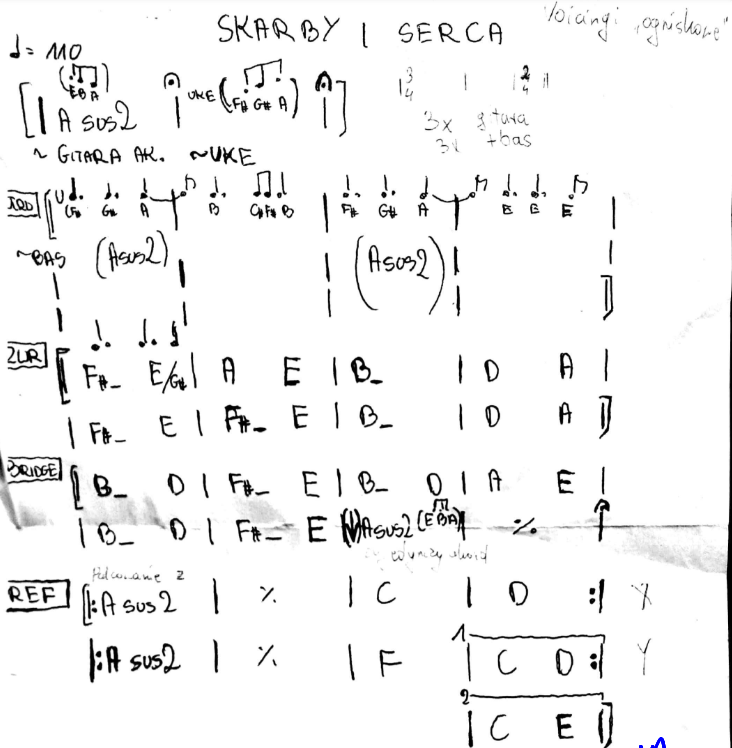
\includegraphics[height=16cm]{images/skarby.png}
    \end{center}
\end{song}

\newpage
\begin{song}{title={Bouda}, music={Zofia Starosta, Mateusz Dorobek}}
    \begin{multicols}{2}
    \begin{verse}
        You got the Bouda, ^{D-7}bouda! \\
        You got the Honkers, ^{B7^{#9b13}}oh yeah! \\
        I got a Feeling, ^{E7^{#9b13}}for ya \\
        I wanna ^{A7^{#9b13}}hold you tight ^{D-7}   $\times 2$ \\
    \end{verse}
    \begin{chorus}
        Whe^{D7^{b9}}rever I s^{G-7}leep \\
        What ever I e^{D-9}at \\
        Whenever I take^{FMaj7} a shit or morning shower \\
        A^{Bb13}da Ada i^{A7^{#9b13}}n my Drea^{D-9}ms

        Whe^{D7^{b9}}rever I g^{G-7}o \\
        C^{G-7}hcę zoba^{A-}czyć j^{Bb}ą \\
        I nie jest ważne c^{B-7^{b5}}o kto inny gada \\
        W mo^{Bb13}je głowie t^{A7^{#9b13}}ylko Ada^{D-9}ms ^{Eb7^{#11}}
    \end{chorus}

    \begin{riff}
        \textit{Jam here in D blues scale and moove your bouda to this chonky chords:}\\
        |:
        \writechord{D-7} |
        \writechord{B7^{#9b13}} |
        \writechord{E7^{#9b13}} |
        \writechord{A7^{#9b13}} :|
        $\times 2137$
    \end{riff}

    \begin{verse}
        You got the Bouda, b^{D-7}ouda! \\
        You got the Honkers, o^{B7^{#9b13}}h yeah! \\
        I got a Feeling, f^{E7^{#9b13}}or ya \\
        I wanna h^{A7^{#9b13}}old you tight $\times 2$ \\
    \end{verse}
    \begin{chorus}
        Whe^{D7^{b9}}rever I s^{G-7}leep \\
        What ever I e^{D-9}at \\
        Whenever I take^{FMaj7} a shit or morning shower \\
        A^{Bb13}da Ada i^{A7^{#9b13}}n my Drea^{D-9}ms

        Whe^{D7^{b9}}rever I g^{G-7}o \\
        C^{G-7}hcę zoba^{A-}czyć j^{Bb}ą \\
        I nie jest ważne c^{B-7^{b5}}o kto inny gada \\
        W mo^{Bb13}je głowie t^{A7^{#9b13}}ylko Ada^{D-9}ms ^{Eb7^{#11}}
    \end{chorus}
\end{multicols}
\end{song}

\chapter{Legendy, opowieści, ciekawostki}
\begin{center}
    \includegraphics[width=0.4\textwidth]{images/bosman.png}
\end{center}
\pagestyle{legendy}
\input{legendy}

% Ostatnia strona parzysta pusta, żeby nie było tekstu na odwrocie
\clearpage{\mbox{}\pagestyle{empty}\cleardoublepage}

\end{document}
